\chapter{因子分解}

\begin{leadbox}
本章では,与えられたデータを複数の要素の積に分解する因子分解技術について説明します.
現実の多くの問題において,一見複雑に見えるデータも,
実は少数の要素(因子・基底とも呼ぶ)の組み合わせで構成されていることが多いのです.
ここでは,非負値行列に対する非負値行列因子分解 (nonnegative matrix factorization, NMF),
ある特殊な形式のテンソル(半正定値行列の集合)に対する
半正定値テンソル分解 (positive semidefinite tensor factorization, PSDTF),
非負値整数行列に対する確率的潜在成分配分法 (probabilistic latent component analysis, PLCA)
について説明します.
また,各手法に対し,確率モデルの最尤推定としての解釈が可能であり,
適切なノンパラメトリックベイズ事前分布を導入することで,
データに合わせて実効的な基底数(要素数)を自動調節できることを解説します.
\end{leadbox}

\section{非負値行列因子分解}
\label{sec:nmf}

非負値行列因子分解 (nonnegative matrix factorization: NMF)\cite{lee:nature:1999,fevotte:neco:2009}は,
音楽音響信号の各フレームのスペクトルを,
少数の基底スペクトルの重み付き線形和で近似するための技術です.
ここで,基底スペクトルは,ある楽器音のある音高の平均的なスペクトルや,
ある打楽器音の平均的なスペクトルに対応していることが期待されています.
すなわち,基底スペクトルは,楽譜上の音符に対応することになり,
音符ごとに音源分離を行ったり,自動採譜を行ううえでNMFは有用です.

NMFは行列分解の一種ですが,
基底スペクトルと重みをいずれも非負値に限定していることが特徴です.
その副次的な効果として,重みがスパースになるよう誘導されます.
なぜなら,重みが非負値に限定されているため,
あるフレームにおいて,いったんある基底スペクトルが利用されると,
他の基底スペクトルを減算することで,その影響を打ち消すことができないからです.
すなわち,利用する基底スペクトルの個数は節約する方がよいということになります.
音響信号全体では$K$個の基底スペクトルが必要であるとしても,
各時間フレームでは限られた少数の基底スペクトルのみが実際に発音しているため,
NMFによるスパース性の誘発は大変都合がよいのです.

この考え方を進めると,入力音響信号に合わせて基底数$K$を手動で調整する代わりに,
可算無限個の基底の存在を仮定し,必要な基底だけが自動的に実体化できれば好都合です.
本章では,NMFに基づく
モノラル音響信号の音源分離について説明します.
まず,コスト関数最小化としての定式化(最尤推定)と音源分離への適用について説明し,
発展的内容としてノンパラメトリックベイズモデルの学習について解説します.

\subsection{コスト関数最小化としての定式化}
\label{sec:nmf_min_cost}

\begin{figure}[t]
\centering
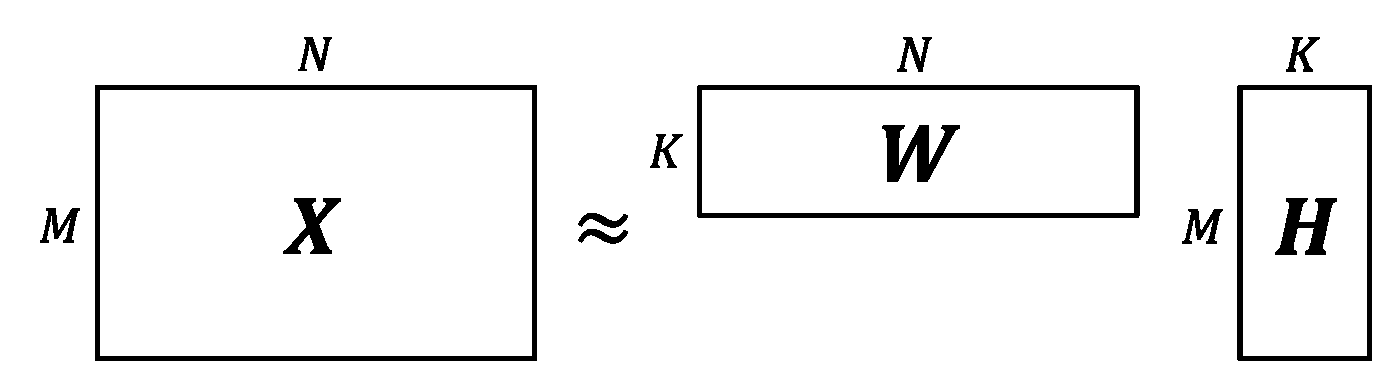
\includegraphics[width=.93\linewidth]{sections/factorization/nmf}
\caption{非負値行列因子分解 (NMF) による低ランク近似.}
\label{fig:nmf}
\end{figure}

NMFでは,非負値行列
$\bm{X} = [\bm{x}_1,\cdots,\bm{x}_N] \in \mathbb{R}_+^{M \times N}$を,
二つの非負値行列$\bm{W} = [\bm{w}_1,\cdots,\bm{w}_K] \in \mathbb{R}_+^{M \times K}$
および$\bm{H} = [\bm{h}_1,\cdots,\bm{h}_K] \in \mathbb{R}_+^{N \times K}$の積である
低ランクな再構成行列$\bm{Y}=\bm{W}\bm{H}^T$で近似します(\figref{fig:nmf}).
\begin{align}
\bm{X} \approx \bm{W}\bm{H}^T \overset{\mbox{\tiny def}}{=} \bm{Y}
\end{align}
ここで,$\bm{w}_k \in \mathbb{R}_+^M$と$\bm{h}_k \in \mathbb{R}_+^N$はそれぞれ
基底ベクトルとアクティベーションベクトルであり,
基底数は$K \ll \mbox{min}(M, N)$とします.
再構成行列を$\bm{Y} = [\bm{y}_1,\cdots,\bm{y}_N] \in \mathbb{R}_+^{M \times N}$とすると,
以下の通り書き直せます.
\begin{align}
 \bm{x}_n \approx \sum_{k=1}^{K} h_{kn} \bm{w}_k \overset{\mbox{\tiny def}}{=} \bm{y}_n
 \label{eqn:x_wh_elem}
\end{align}

\begin{figure}[t]
\centering
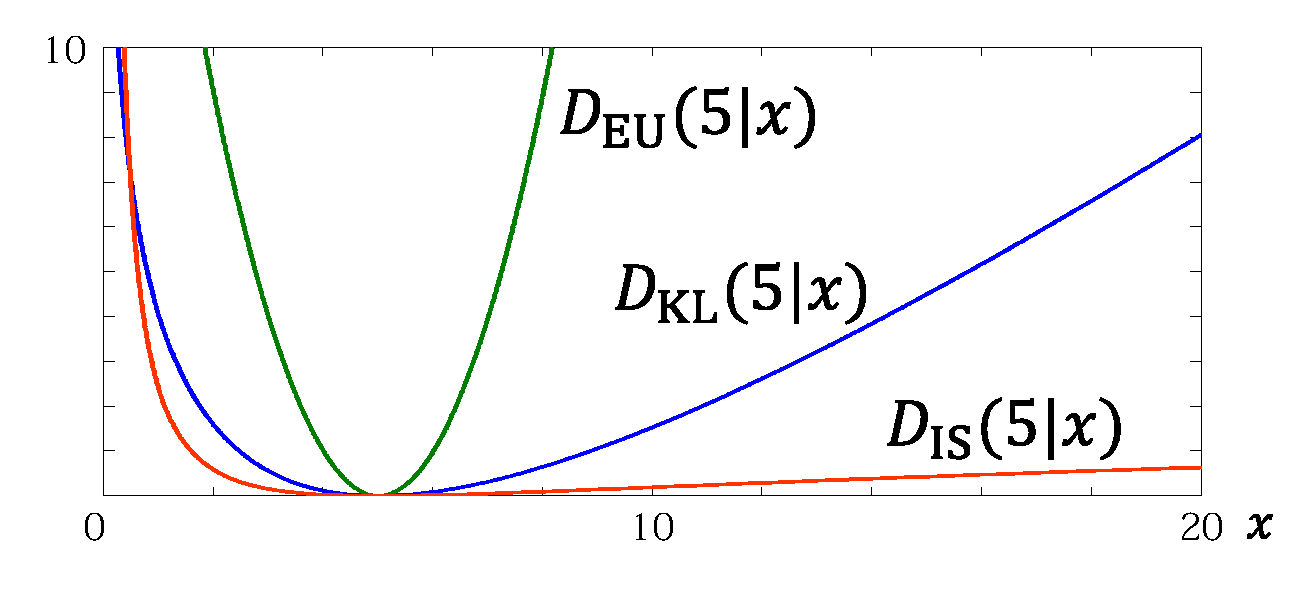
\includegraphics[width=.9\linewidth]{sections/factorization/cost_functions}
\vspace{-2mm}
\caption{ユークリッド距離,KLダイバージェンス,ISダイバージェンスに基づくコスト関数$D(5|x)$.
ユークリッド距離以外は$x=5$の左右で非対称であることに注意.}
\label{fig:cost_functions}
\end{figure}

NMFでは,観測データ$\bm{X}$が与えられたときに,
コスト関数
\begin{align}
\mathcal{D}(\bm{X}|\bm{Y}) = \sum_{n=1}^N \mathcal{D}(\bm{x}_n|\bm{y}_n)
\end{align}
を最小化する$\bm{Y}$($\bm{W}$および$\bm{H}$)を求めます.
非負値の観測ベクトル$\bm{x}_n$と非負値の再構成ベクトル$\bm{y}_n$との間の
誤差$\mathcal{D}(\bm{x}_n|\bm{y}_n)$が小さいほど,低ランク近似の精度がよいことになります.

誤差$\mathcal{D}(\bm{x}_n|\bm{y}_n)$を評価する尺度として,ユークリッド距離,
一般化Kullback-Leibler (KL) ダイバージェンス\cite{smaragdis:waspaa:2003},
およびItakura-Saito (IS) ダイバージェンス\cite{fevotte:neco:2009}などがよく利用されています.
\begin{align}
&\mathcal{D}_{\mbox{\tiny EU}}(\bm{x}_n|\bm{y}_n)
= \sum_{m=1}^M \! \left(x_{nm} - {y_{nm}}\right)^2
\!\!\!
\label{eqn:nmf_kl}
\\
&\mathcal{D}_{\mbox{\tiny KL}}(\bm{x}_n|\bm{y}_n)
= \sum_{m=1}^M \! \left(x_{nm}\log\frac{x_{nm}}{y_{nm}} - x_{nm} + {y_{nm}}\right)
\!\!\!
\label{eqn:nmf_kl}
\\
& \mathcal{D}_{\mbox{\tiny IS}}(\bm{x}_n|\bm{y}_n) 
= \sum_{m=1}^M \! \left(\frac{x_{nm}}{y_{nm}} - \log \frac{x_{nm}}{y_{nm}} - 1\right)
\!\!\!
\label{eqn:nmf_is}
\end{align}
例として,\figref{fig:cost_functions}に,
$\bm{x}_n$および$\bm{y}_n$がいずれもスカラ(1次元のベクトル)である場合のコスト関数の値を示します.
これらの関数は常に非負値をとり,$\bm{x}_n = \bm{y}_n$のときのみ0となります.

KLダイバージェンスとISダイバージェンスは,
ユークリッド距離などの通常の距離尺度と異なり,非対称性をもっています.
\begin{align}
\mathcal{D}_{\mbox{\tiny EU}}(\bm{x}_n|\bm{y}_n) &=   \mathcal{D}_{\mbox{\tiny EU}}(\bm{y}_n|\bm{x}_n)\\
\mathcal{D}_{\mbox{\tiny KL}}(\bm{x}_n|\bm{y}_n) &\ne \mathcal{D}_{\mbox{\tiny KL}}(\bm{y}_n|\bm{x}_n)\\
\mathcal{D}_{\mbox{\tiny IS}}(\bm{x}_n|\bm{y}_n) &\ne \mathcal{D}_{\mbox{\tiny IS}}(\bm{y}_n|\bm{x}_n)
\end{align}
\figref{fig:cost_functions}に示す通り,ユークリッド距離は,$x=5$の左右で対称な二次関数ですが,
KLダイバージェンスやISダイバージェンスは,$x=5$から離れるにつれて,
$x<5$よりも$x>5$の方が値の増加がはるかに緩やかな関数であることが分かります.

また,これらの中では,
ISダイバージェンスのみがスケール不変性を持っています.
すなわち,任意の実数$\alpha>0$に対して,以下が成立します.
\begin{align}
\mathcal{D}_{\mbox{\tiny EU}}(\bm{x}_n|\bm{y}_n) &\ne \mathcal{D}_{\mbox{\tiny EU}}(\alpha \bm{x}_n | \alpha \bm{y}_n)\\
\mathcal{D}_{\mbox{\tiny KL}}(\bm{x}_n|\bm{y}_n) &\ne \mathcal{D}_{\mbox{\tiny KL}}(\alpha \bm{x}_n | \alpha \bm{y}_n)\\
\mathcal{D}_{\mbox{\tiny IS}}(\bm{x}_n|\bm{y}_n) &=   \mathcal{D}_{\mbox{\tiny IS}}(\alpha \bm{x}_n | \alpha \bm{y}_n)
\end{align}
音響信号に対してNMFを適用するうえで,スケール不変性は重要な性質です.
スケール不変性を持たない場合には,
音楽音響信号全体の音量を変化させただけで,
NMFで得られる結果が異なってしまいます.
そのため,理論的にはISダイバージェンスが妥当ですが,
経験的にはKLダイバージェンスが安定してよい結果を与えることが知られています.

\subsection{乗法更新アルゴリズムに基づく最適化}
\label{sec:nmf_mu}

コスト関数$\mathcal{D}(\bm{X}|\bm{Y})$
を最小化する$\bm{Y}$を直接求めることは困難なため,
乗法更新則 (multiplicative updating rules) に基づく
反復最適化技法が提案されています\cite{kameoka:asjj:2012}.
本節では,補助関数法(付録\ref{sec:aux}節)に基づく収束性が保証された乗法更新則を紹介します.
具体的には,コスト関数$\mathcal{D}(\bm{X}|\bm{Y})$の上限関数$\mathcal{U}(\bm{X}|\bm{Y},\bm\Theta)$を設計し,
$\bm{Y}$と$\bm\Theta$について交互に逐次最小化することで,
間接的に$\mathcal{D}(\bm{X}|\bm{Y})$を逐次最小化します.
ここで,$\bm\Theta$は新たに導入された補助変数であり,
$\mathcal{U}(\bm{X}|\bm{Y},\bm\Theta)$を$\bm\Theta$について最小化することで,
もとの関数$\mathcal{D}(\bm{X}|\bm{Y})$と同じ値をとるようにしておく必要があります.
\begin{align}
\mathcal{D}(\bm{X}|\bm{Y}) = \min_{\bm\Theta} \mathcal{U}(\bm{X}|\bm{Y},\bm\Theta)
\end{align}

効率的な乗法更新則を導出するうえで,
$\mathcal{U}(\bm{X}|\bm{Y},\bm\Theta)$は,
$\bm{Y}$と$\bm\Theta$のいずれに関しても,一方が既知であれば,
もう一方に関する最小化を容易に行えることが重要です.
特に,$\bm{Y}$と$\bm\Theta$の更新則がいずれも閉形式で記述できることが理想です.
そうでないと,$\bm{Y}$と$\bm\Theta$を更新する1ステップ内においてすら,
最急降下法や(準)ニュートン法などを利用した反復最適化が必要になり,
数値的安定性・計算量・収束性などに問題が発生することがあります.

\subsection{EU-NMFの乗法更新アルゴリズム}

ユークリッド距離に基づくNMF (EU-NMF) の乗法更新則を導出します.
準備として,二次関数が下に凸であることから,
Jensenの不等式(付録\ref{sec:jensen}節)を用いて,
$f(\bm{z}) = \left(\sum_{k=1}^K z_k\right)^2$の
上限関数$u(\bm{z},\bm\lambda)$を設計します.
\begin{align}
f(\bm{z}) 
= \left(\sum_{k=1}^K \lambda_k \frac{z_k}{\lambda_k}\right)^2
\le \sum_{k=1}^K \lambda_k \left(\frac{z_k}{\lambda_k}\right)^2
= \sum_{k=1}^K \frac{z_k^2}{\lambda_k}
\overset{\mbox{\scriptsize{def}}}{=}
u(\bm{z},\bm\lambda)
\label{eqn:quad_aux}
\end{align}
ここで,$z_k \ge 0$は非負値の変数であり,
$\bm\lambda = \{\lambda_k\}_{k=1}^K$は
\begin{align}
\sum_{k=1}^K \lambda_k = 1
\label{eqn:eu_lambda_constraint}
\end{align}
を満たす非負値の補助変数です.
「和の二次関数」の上限関数として,
「二次関数の和」が得られていることに注意してください.
Jensenの不等式を用いると,和と凸関数(あるいは凹関数)の適用順序を交換できます.

等号成立条件,すなわち,
\refeq{eqn:eu_lambda_constraint}の制約条件付きで
$u(\bm{z},\bm\lambda)$を最小化する$\bm\lambda$を求めるには,
ラグランジュの未定乗数法を用います.
まず,未定乗数$\phi$を用いて,新たな関数
\begin{align}
F(\bm\lambda,\phi) = \sum_{k=1}^K \frac{z_k^2}{\lambda_k} + \phi \left(1 - \sum_{k=1}^K \lambda_k\right)
\end{align}
を考えます.ここで,$\bm\lambda$が制約条件を満たす場合には,
第二項は$0$であることに注意してください.
これを$\lambda_k$について偏微分すると
\begin{align}
\frac{\partial F(\bm\lambda,\phi)}{\partial\lambda_k} = - \frac{z_k^2}{\lambda_k^2} - \phi
\end{align}
を得ます.$\frac{\partial F(\bm\lambda,\phi)}{\partial\lambda_k} = 0$とおくと,
$\phi$を用いて$\lambda_k$が表せます.
\begin{align}
\lambda_k = \frac{z_k}{\sqrt{-\phi}}
\label{eqn:lambda_k_eu_nmf}
\end{align}
これを\refeq{eqn:eu_lambda_constraint}に代入すると,
\begin{align}
1 = \sum_{k=1}^K \lambda_k = \frac{1}{\sqrt{-\phi}}\sum_{k=1}^K z_k
\end{align}
となるので,未定乗数$\phi$は
\begin{align}
\sqrt{-\phi} = \sum_{k=1}^K z_k
\end{align}
で与えられます.これを,\refeq{eqn:lambda_k_eu_nmf}に代入すると,次式を得ます.
\begin{align}
\lambda_k = \frac{z_k}{\sum_{k=1}^K z_k}
\end{align}

この結果を用いて,コスト関数$\mathcal{D}(\bm{X}|\bm{Y})$に対して,
補助変数$\bm\lambda$を含む上限関数$\mathcal{U}(\bm{X}|\bm{Y},\bm\lambda)$を導出します.
\begin{align}
\mathcal{D}(\bm{X}|\bm{Y}) 
&= \sum_{n=1}^N \sum_{m=1}^M \left(x_{nm} - y_{nm}\right)^2
\nonumber\\
&= \sum_{n=1}^N \sum_{m=1}^M \left(x_{nm}^2 - 2 x_{nm} \sum_{k=1}^K w_{km}h_{kn} + \left(\sum_{k=1}^K w_{km} h_{kn}\right)^2\right)
\nonumber\\
&\le \sum_{n=1}^N \sum_{m=1}^M \left(x_{nm}^2 - 2 x_{nm} \sum_{k=1}^K w_{km}h_{kn} 
   + \sum_{k=1}^K \frac{w_{km}^2 h_{kn}^2}{\lambda_{nmk}}\right)
\nonumber\\
&\overset{\mbox{\scriptsize{def}}}{=} \mathcal{U}(\bm{X}|\bm{Y},\bm\lambda)
\label{eqn:eu_nmf_u}
\end{align}
ここで,\refeq{eqn:quad_aux}を用いました.
補助変数$\bm\lambda=\{\lambda_{nmk}\}_{n=1,m=1,k=1}^{N,M,K}$は,
$\sum_{k=1}^K \lambda_{nmk} = 1$を満たします.
また,等号成立条件,
すなわち$\mathcal{U}(\bm{X}|\bm{Y},\bm\lambda)$を最小化する$\bm\lambda$は次式で与えられます.
\begin{align}
\lambda_{nmk} 
= \frac{w_{km}h_{kn}}{\sum_{k'=1}^K w_{k'm}h_{k'n}}
= \frac{w_{km}h_{kn}}{y_{nm}}
\label{eqn:eu_nmf_mu_lambda}
\end{align}

最後に,\refeq{eqn:eu_nmf_u}を最小化する$\bm{Y}$($\bm{W}$および$\bm{H}$)を求めます.
まず,$\mathcal{U}(\bm{X}|\bm{Y},\bm\lambda)$を$w_{km}$について偏微分すると,
\begin{align}
\frac{\partial \mathcal{U}(\bm{X}|\bm{Y},\bm\lambda)}{\partial w_{km}} 
= \sum_{n=1}^N \left(- 2 x_{nm} h_{kn} + \frac{2 w_{km} h_{kn}^2}{\lambda_{nmk}}\right)
\end{align}
を得ます.
ここで,$\frac{\partial \mathcal{U}(\bm{X}|\bm{Y},\bm\lambda)}{\partial w_{km}}=0$とおくと,
\begin{align}
w_{km} 
= \frac{\sum_{n=1}^N x_{nm} h_{kn}}{\sum_{n=1}^N \frac{h_{kn}^2}{\lambda_{nmk}}}
\label{eqn:eu_nmf_mu_w}
\end{align}
を得ます.同様に,$\mathcal{U}(\bm{X}|\bm{Y},\bm\lambda)$を$h_{kn}$について偏微分して$0$とおくことで,
\begin{align}
h_{kn} 
= \frac{\sum_{m=1}^M x_{nm} w_{km}}{\sum_{m=1}^M \frac{w_{km}^2}{\lambda_{nmk}}}
\label{eqn:eu_nmf_mu_h}
\end{align}
を得ます.
\refeq{eqn:eu_nmf_mu_lambda},\refeq{eqn:eu_nmf_mu_w}および
\refeq{eqn:eu_nmf_mu_h}は互いに依存関係にあり,
$\mathcal{U}(\bm{X}|\bm{Y},\bm\lambda)$を最小化する$\bm\lambda$,$\bm{W}$および$\bm{H}$を
一挙に求めることができません.
そのため,これらの式を交互に反復計算することにより,
徐々に\refeq{eqn:eu_nmf_u}を小さくしていくことになります.

NMFの乗法更新則は,補助変数を介さずに表現することもできます.
具体的には,\refeq{eqn:eu_nmf_mu_lambda}を\refeq{eqn:eu_nmf_mu_w}および
\refeq{eqn:eu_nmf_mu_h}に代入することで,
\begin{align}
&w_{km} 
\gets \frac{\sum_{n=1}^N x_{nm} h_{kn}}{\sum_{n=1}^N \frac{h_{kn}^2}{\lambda_{nmk}}}
= \frac{\sum_{n=1}^N x_{nm} h_{kn}}{\sum_{n=1}^N \frac{y_{nm} h_{kn}}{w_{km}}}
= \frac{\sum_{n=1}^N x_{nm} h_{kn}}{\sum_{n=1}^N y_{nm} h_{kn}} w_{km}
\label{eqn:eu_nmf_mu_w2}
\\
& h_{kn}
\gets \frac{\sum_{m=1}^M x_{nm} w_{km}}{\sum_{m=1}^M \frac{w_{km}^2}{\lambda_{nmk}}}
%= \frac{\sum_{m=1}^M x_{nm} w_{km}}{\sum_{m=1}^M \frac{y_{nm} w_{km}}{h_{kn}}}
= \frac{\sum_{m=1}^M x_{nm} w_{km}}{\sum_{m=1}^M y_{nm} w_{km}} h_{kn}
\label{eqn:eu_nmf_mu_h2}
\end{align}
を得ます.
ここで,記号$\gets$は,右辺値を左辺値に代入して更新するという意味です.
$\gets$の右側においては,
$\bm\lambda$,$\bm{W}$および$\bm{H}$の更新前の古い値を用います.
同じ変数が$\gets$の左右に登場すると混乱するため,
等号ではなく,記号$\gets$を用いています.

これらが「乗法」更新則と呼ばれる所以は,
自分自身に係数を掛け合わせて更新を行うからです.
例えば,\refeq{eqn:eu_nmf_mu_w2}では,
$w_{km}$に係数$\frac{\sum_{n=1}^N x_{nm} h_{kn}}{\sum_{n=1}^N y_{nm} h_{kn}} \ge 0 $を掛け合わせています.
このとき,係数も非負値であることから,特別な制約を導入しなくても,
$w_{km}$の非負値性は自然に保たれます.
また,$w_{km}=0$として初期化すると,
以降の更新では常に$w_{km}=0$が維持されます.

\refeq{eqn:eu_nmf_mu_w2}および\refeq{eqn:eu_nmf_mu_h2}は,
行列演算を用いて簡潔に書けます.
\begin{align}
\bm{W} \gets \frac{\bm{H}\bm{X}^T}{\bm{H}\bm{Y}^T} \odot \bm{W}
\label{eqn:eu_nmf_mu_W}
\\
\bm{H} \gets \frac{\bm{W}\bm{X}}{\bm{W}\bm{Y}} \odot \bm{H}
\label{eqn:eu_nmf_mu_H}
\end{align}
ここで,割り算---や掛け算$\odot$は行列の各要素ごとに行うものとします.
高速な行列演算が可能なプログラミング言語(例:MATLAB)では,
for文を使わずに上記の更新式を直接コーディングすることができ,
CPUやGPUのベクトル演算機能を利用した高速な更新が可能になります.

\refalgo{algo:eu-nmf-ml}に,EU-NMFのアルゴリズムを示します
(これが実は,ある確率モデルの最尤推定になっていることはあとで示します).
このアルゴリズムは山登り法(NMFではコスト関数を最小化しているので実際には「山下り法」)の一種であり,
大域的な最適解を見つけられる保証はなく,
得られる結果は$\bm{W}$および$\bm{H}$の初期値に大きな影響を受けます.
また,スケールの任意性を解消するため,
$\sum_{m=1}^M w_{km} = 1$を満たすように正規化しておくことにします.
具体的には,$w_{km}$を更新した結果,$\sum_{m=1}^M w_{km} = s$になってしまったとすると,
すべての$m,n$について$w_{km} \gets \frac{1}{s} w_{km}$および
$h_{kn} \gets s h_{kn}$と更新しておきます.
この処理ではコスト関数の値は変化しません.
$\sum_{n=1}^N h_{kn} = 1$となるようアクティベーションを正規化することもできますが,
基底ベクトルを正規化しておくのが一般的です.
\begin{algobox}{EU-NMFの最尤推定}
\label{algo:eu-nmf-ml}
\begin{algorithmic}[1]
\Require 非負値行列$\bm{X} \in \mathbb{R}_+^{M \times N}$, 基底数$K$
\State 非負値行列$\bm{W} \in \mathbb{R}_+^{M \times K}$をランダムに初期化
\State 非負値行列$\bm{H} \in \mathbb{R}_+^{M \times K}$をランダムに初期化
\While{上限関数$\mathcal{U}(\bm{X}|\bm{Y},\bm\lambda)$が未収束}
\State $\displaystyle \bm{W} \gets \frac{\bm{H}\bm{X}^T}{\bm{H}\bm{Y}^T} \odot \bm{W}$ 
\State $\displaystyle \bm{H} \gets \frac{\bm{W}\bm{X}}{\bm{W}\bm{Y}} \odot \bm{H}$ 
\EndWhile\\
{\bf Return} 非負値行列$\bm{W}$, $\bm{H}$
\end{algorithmic}
\end{algobox}

\subsection{KL-NMFの乗法更新アルゴリズム}

EU-NMFとほとんど同様の方法で,
KLダイバージェンスに基づくNMF (KL-NMF) の乗法更新則を導出することができます.
準備として,負の対数関数が下に凸であることから,
Jensenの不等式(付録\ref{sec:jensen}節)を用いて,
$f(\bm{z}) = - \log \left(\sum_{k=1}^K z_k \right)$の
上限関数$u(\bm{z},\bm\lambda)$を設計します.
\begin{align}
f(\bm{z})
= - \log \left(\sum_{k=1}^K \lambda_k \frac{z_k}{\lambda_k}\right)
\le - \sum_{k=1}^K \lambda_k \log \frac{z_k}{\lambda_k}
\overset{\mbox{\scriptsize{def}}}{=}
u(\bm{z},\bm\lambda)
\label{eqn:log_aux}
\end{align}
ここで,$z_k \ge 0$は非負値の変数であり,
$\bm\lambda = \{\lambda_k\}_{k=1}^K$は
\begin{align}
\sum_{k=1}^K \lambda_k = 1
\label{eqn:kl_lambda_constraint}
\end{align}
を満たす非負値の補助変数です.
「和の対数関数」の上限関数として,
「対数関数の和」が得られていることに注意してください.

等号成立条件,すなわち,
\refeq{eqn:kl_lambda_constraint}の制約条件付きで
$u(\bm{z},\bm\lambda)$を最小化する$\bm\lambda$を求めるには,
ラグランジュの未定乗数$\phi$を用いて,新たな関数
\begin{align}
F(\bm\lambda,\phi) = \sum_{k=1}^K \lambda_k \log \frac{z_k}{\lambda_k} + \phi \left(1 - \sum_{k=1}^K \lambda_k\right)
\end{align}
を考えます.これを$\lambda_k$について偏微分すると
\begin{align}
\frac{\partial F(\bm\lambda,\phi)}{\partial\lambda_k} 
= \log z_k - \log \lambda_k - 1 - \phi
\end{align}
を得ます.$\frac{\partial F(\bm\lambda,\phi)}{\partial\lambda_k} = 0$とおくと,
$\phi$を用いて$\lambda_k$が表せます.
\begin{align}
\lambda_k = \frac{z_k}{e^{1+\phi}}
\label{eqn:lambda_k_kl_nmf}
\end{align}
これを\refeq{eqn:kl_lambda_constraint}に代入すると,
\begin{align}
1 = \sum_{k=1}^K \lambda_k = \frac{1}{e^{1+\phi}}\sum_{k=1}^K z_k
\end{align}
となるので,未定乗数$\phi$は
\begin{align}
e^{1+\phi} = \sum_{k=1}^K z_k
\end{align}
で与えられます.これを,\refeq{eqn:lambda_k_kl_nmf}に代入すると,次式を得ます.
\begin{align}
\lambda_k = \frac{z_k}{\sum_{k=1}^K z_k}
\end{align}

この結果を用いて,コスト関数$\mathcal{D}(\bm{X}|\bm{Y})$に対して,
補助変数$\bm\lambda$を含む上限関数$\mathcal{U}(\bm{X}|\bm{Y},\bm\lambda)$を導出します.
\begin{align}
\mathcal{D}(\bm{X}|\bm{Y}) 
&= \sum_{n=1}^N \sum_{m=1}^M \left(x_{nm} \log x_{nm} - x_{nm} \log y_{nm} - x_{nm} + y_{nm}\right)
\nonumber\\
&\overset{c}{=} \sum_{n=1}^N \sum_{m=1}^M \left(- x_{nm} \log \sum_{k=1}^K w_{km}h_{kn} + \sum_{k=1}^K w_{km}h_{kn}\right)
\nonumber\\
&\le \sum_{n=1}^N \sum_{m=1}^M \left(- x_{nm} \sum_{k=1}^K \lambda_{nmk} \log \frac{w_{km}h_{kn}}{\lambda_{nmk}} + \sum_{k=1}^K w_{km}h_{kn}\right)
\nonumber\\
&\overset{\mbox{\scriptsize{def}}}{=} \mathcal{U}(\bm{X}|\bm{Y},\bm\lambda)
\label{eqn:kl_nmf_u}
\end{align}
ここで,
%定数項を除いて等しいことを表す記号$\overset{c}{=}$を導入し
%(観測データ$x_{nm}$は既知なので定数項),
\refeq{eqn:log_aux}を用いました.
また,補助変数$\bm\lambda$は,
$\sum_{k=1}^K \lambda_{nmk} = 1$を満たすものとします.
等号成立条件,
すなわち$\mathcal{U}(\bm{X}|\bm{Y},\bm\lambda)$を最小化する$\bm\lambda$は次式で与えられます.
\begin{align}
\lambda_{nmk} 
= \frac{w_{km}h_{kn}}{\sum_{k'=1}^K w_{k'm}h_{k'n}}
= \frac{w_{km}h_{kn}}{y_{nm}}
\label{eqn:kl_nmf_mu_lambda}
\end{align}

最後に,\refeq{eqn:kl_nmf_u}を最小化する$\bm{Y}$($\bm{W}$および$\bm{H}$)を求めます.
まず,$\mathcal{U}(\bm{X}|\bm{Y},\bm\lambda)$を$w_{km}$について偏微分すると,
\begin{align}
\frac{\partial \mathcal{U}(\bm{X}|\bm{Y},\bm\lambda)}{\partial w_{km}} 
= \sum_{n=1}^N \left(- \frac{x_{nm} \lambda_{nmk}}{w_{km}} + h_{kn} \right)
\end{align}
を得ます.
ここで,$\frac{\partial \mathcal{U}(\bm{X}|\bm{Y},\bm\lambda)}{\partial w_{km}}=0$とおくと,
\begin{align}
w_{km} 
= \frac{\sum_{n=1}^N x_{nm} \lambda_{nmk}}{\sum_{n=1}^N h_{kn}}
\label{eqn:kl_nmf_mu_w}
\end{align}
を得ます.同様に,$\mathcal{U}(\bm{X}|\bm{Y},\bm\lambda)$を$h_{kn}$について偏微分して$0$とおくことで,
\begin{align}
h_{kn} 
= \frac{\sum_{m=1}^M x_{nm} \lambda_{nmk}}{\sum_{m=1}^M w_{km}}
\label{eqn:kl_nmf_mu_h}
\end{align}
を得ます.
EU-NMFと同様に,
\refeq{eqn:kl_nmf_mu_lambda},\refeq{eqn:kl_nmf_mu_w}および\refeq{eqn:kl_nmf_mu_h}
を反復することにより,
$\mathcal{U}(\bm{X}|\bm{Y},\bm\lambda)$を逐次最小化していくことができます.

補助変数を介さない乗法更新則は,
\refeq{eqn:kl_nmf_mu_lambda}を\refeq{eqn:kl_nmf_mu_w}および\refeq{eqn:kl_nmf_mu_h}
に代入することで得られます.
\begin{align}
w_{km} 
&\gets \frac{\sum_{n=1}^N x_{nm} \frac{w_{km} h_{kn}}{y_{nm}}}{\sum_{n=1}^N h_{kn}}
= \frac{\sum_{n=1}^N h_{kn} \frac{x_{nm}}{y_{nm}}}{\sum_{n=1}^N h_{kn}} w_{km}
\label{eqn:kl_nmf_mu_w2}
\\
h_{kn} 
&\gets \frac{\sum_{m=1}^M x_{nm} \frac{w_{km} w_{km}}{y_{nm}}}{\sum_{m=1}^M w_{km}}
= \frac{\sum_{m=1}^M w_{km} \frac{x_{nm}}{y_{nm}}}{\sum_{m=1}^M w_{kn}} h_{kn}
\label{eqn:kl_nmf_mu_h2}
\end{align}
全要素が$1$の行列を$\bm{1} \in \mathbb{R}^{M \times N}$とすると,
行列演算として記述できます.
\begin{align}
\bm{W} \gets \frac{\bm{H} \frac{\bm{X}^T}{\bm{Y}^T}}{\bm{H}\bm{1}^T} \odot \bm{W}
\label{eqn:kl_nmf_mu_W}
\\
\bm{H} \gets \frac{\bm{W} \frac{\bm{X}}{\bm{Y}}}{\bm{W}\bm{1}} \odot \bm{H}
\label{eqn:kl_nmf_mu_H}
\end{align}

\begin{algobox}{KL-NMFの最尤推定}
\label{algo:kl-nmf-ml}
\begin{algorithmic}[1]
\Require 非負値行列$\bm{X} \in \mathbb{R}_+^{M \times N}$, 基底数$K$
\State 非負値行列$\bm{W} \in \mathbb{R}_+^{M \times K}$をランダムに初期化
\State 非負値行列$\bm{H} \in \mathbb{R}_+^{M \times K}$をランダムに初期化
\While{上限関数$\mathcal{U}(\bm{X}|\bm{Y},\bm\lambda)$が未収束}
\State $\displaystyle \bm{W} \gets \frac{\bm{H} \frac{\bm{X}^T}{\bm{Y}^T}}{\bm{H}\bm{1}^T} \odot \bm{W}$ 
\State $\displaystyle \bm{H} \gets \frac{\bm{W} \frac{\bm{X}}{\bm{Y}}}{\bm{W}\bm{1}} \odot \bm{H}$ 
\EndWhile\\
{\bf Return} 非負値行列$\bm{W}$, $\bm{H}$
\end{algorithmic}
\end{algobox}
\refalgo{algo:kl-nmf-ml}に,KL-NMFのアルゴリズムを示します.
これも,EU-NMFと同様に,ある確率モデルの最尤推定としての解釈が可能です.

\subsection{IS-NMFの乗法更新アルゴリズム}

ISダイバージェンスに基づくNMF (IS-NMF) の乗法更新則を導出します.
準備として,逆数関数が下に凸であることから,
Jensenの不等式(付録\ref{sec:jensen}節)を用いて,
$f(\bm{z})=\frac{1}{\left(\sum_{k=1}^K z_k \right)}$
の上限関数$u(\bm{z},\bm\lambda)$を設計します.
\begin{align}
f(\bm{z}) 
= \frac{1}{\left(\sum_{k=1}^K \lambda_k \frac{z_k}{\lambda_k} \right)}
\le \sum_{k=1}^K \lambda_k \frac{1}{\frac{z_k}{\lambda_k}}
= \sum_{k=1}^K \lambda_k^2 \frac{1}{z_k}
\overset{\mbox{\scriptsize{def}}}{=}
u(\bm{z},\bm\lambda)
\label{eqn:inv_aux}
\end{align}
ここで,$z_k \ge 0$は非負値の変数であり,
$\bm\lambda = \{\lambda_k\}_{k=1}^K$は
\begin{align}
\sum_{k=1}^K \lambda_k = 1
\label{eqn:is_lambda_constraint}
\end{align}
を満たす非負値の補助変数です.
「和の逆数関数」の上限関数として,
「逆数関数の和」が得られていることに注意してください.

等号成立条件,すなわち,
\refeq{eqn:is_lambda_constraint}の制約条件付きで
$u(\bm{z},\bm\lambda)$を最小化する$\bm\lambda$を求めるには,
未定乗数$\phi$を用いて,新たな関数
\begin{align}
F(\bm\lambda,\phi) = \sum_{k=1}^K \lambda_k^2 \frac{1}{z_k} + \phi \left(1 - \sum_{k=1}^K \lambda_k\right)
\end{align}
を考えます.これを$\lambda_k$について偏微分すると
\begin{align}
\frac{\partial F(\bm\lambda,\phi)}{\partial\lambda_k} 
= \frac{2 \lambda_k}{z_k} - \phi
\end{align}
を得ます.$\frac{\partial F(\bm\lambda,\phi)}{\partial\lambda_k} = 0$とおくと,
$\phi$を用いて$\lambda_k$が表せます.
\begin{align}
\lambda_k = \frac{\phi}{2} z_k
\label{eqn:lambda_k_is_nmf}
\end{align}
これを\refeq{eqn:is_lambda_constraint}に代入すると,
\begin{align}
1 = \sum_{k=1}^K \lambda_k = \frac{\phi}{2}\sum_{k=1}^K z_k
\end{align}
となるので,未定乗数$\phi$は
\begin{align}
\frac{2}{\phi} = \sum_{k=1}^K z_k
\end{align}
で与えられます.これを,\refeq{eqn:lambda_k_is_nmf}に代入すると,次式を得ます.
\begin{align}
\lambda_k = \frac{z_k}{\sum_{k=1}^K z_k}
\end{align}

さらに,対数関数$f(z)=\log(z)$の上限関数$u(z,\omega)$を設計します.
対数関数は上に凸であることから,任意の点$\omega > 0$における接線は
常に対数関数の上側にあります.
したがって,$\omega$における一次のテイラー展開を行うと,
\begin{align}
f(z) \le \log \omega + \frac{z}{\omega} - 1
\overset{\mbox{\scriptsize{def}}}{=}
u(z,\omega)
\label{eqn:log_tangent_aux}
\end{align}
を得ます.
等号成立条件,すなわち,
$u(z,\omega)$を最小化する$\omega$は,
$u(z,\omega)$を$\omega$で偏微分して$0$とおくことで求まります.
\begin{align}
 \omega = x
\end{align}

これらの結果を用いて,コスト関数$\mathcal{D}(\bm{X}|\bm{Y})$に対して,
補助変数$\bm\lambda$および$\bm\omega$を含む上限関数$\mathcal{U}(\bm{X}|\bm{Y},\bm\lambda,\bm\omega)$を導出します.
\begin{align}
\mathcal{D}(\bm{X}|\bm{Y}) 
&= \sum_{n=1}^N \sum_{m=1}^M \left(\frac{x_{nm}}{y_{nm}} - \log \frac{x_{nm}}{y_{nm}} - 1\right)
\nonumber\\
&= \sum_{m=1}^M \left(\frac{x_{nm}}{\sum_{k=1}^K w_{km} h_{kn}} - \log \frac{x_{nm}}{\sum_{k=1}^K w_{km} h_{kn}} - 1\right)
\nonumber\\
&\overset{c}{=}  \sum_{m=1}^M \left(\frac{x_{nm}}{\sum_{k=1}^K w_{km} h_{kn}} + \log \sum_{k=1}^K w_{km} h_{kn} \right)
\nonumber\\
&\le \sum_{n=1}^N \sum_{m=1}^M \left(\sum_{k=1}^K \frac{x_{nm} \lambda_{nmk}^2}{w_{km} h_{kn}} 
+ \log \omega_{nm} + \frac{1}{\omega_{nm}}\sum_{k=1}^K w_{km} h_{kn} - 1\right)
\nonumber\\
&\overset{\mbox{\scriptsize{def}}}{=} \mathcal{U}(\bm{X}|\bm{Y},\bm\lambda,\bm\omega)
\label{eqn:is_nmf_u}
\end{align}
ここで,\refeq{eqn:inv_aux}および\refeq{eqn:log_tangent_aux}を用いました.
補助変数に関しては,$\bm\lambda=\{\lambda_{nmk}\}_{n=1,m=1,k=1}^{N,M,K}$は
$\sum_{k=1}^K \lambda_{nmk} = 1$を満たし,
$\bm\omega=\{\omega_{nm}\}_{n=1,m=1}^{N,M}$はすべて非負値とします.
等号成立条件,
すなわち$\mathcal{U}(\bm{X}|\bm{Y},\bm\lambda,\bm\omega)$を最小化する$\bm\lambda$および$\bm\omega$は次式で与えられます.
\begin{align}
\lambda_{nmk} 
&= \frac{w_{km}h_{kn}}{\sum_{k'=1}^K w_{k'm}h_{k'n}}
= \frac{w_{km}h_{kn}}{y_{nm}}
\label{eqn:is_nmf_mu_lambda}
\\
\omega_{nm} 
&= \sum_{k=1}^K w_{km} h_{kn} = y_{nm}
\label{eqn:is_nmf_mu_omega}
\end{align}

最後に,\refeq{eqn:is_nmf_u}を最小化する$\bm{Y}$($\bm{W}$および$\bm{H}$)を求めます.
まず,$\mathcal{U}(\bm{X}|\bm{Y},\bm\lambda,\bm\omega)$を$w_{km}$について偏微分すると,
\begin{align}
\frac{\partial \mathcal{U}(\bm{X}|\bm{Y},\bm\lambda,\bm\omega)}{\partial w_{km}} 
= \sum_{n=1}^N \left(- \frac{x_{nm}\lambda_{nmk}^2}{w_{km}^2 h_{kn}} + \frac{h_{kn}}{\omega_{nm}}\right)
\end{align}
を得ます.
ここで,$\frac{\partial \mathcal{U}(\bm{X}|\bm{Y},\bm\lambda.\bm\omega)}{\partial w_{km}}=0$とおくと,
\begin{align}
w_{km} 
= \sqrt{
       \frac{\sum_{n=1}^N \frac{x_{nm} \lambda_{nmk}^2}{h_{kn}}}
       {\sum_{n=1}^N \frac{h_{kn}}{\omega_{nm}}}
  }
\label{eqn:is_nmf_mu_w}
\end{align}
を得ます.同様に,$\mathcal{U}(\bm{X}|\bm{Y},\bm\lambda,\bm\omega)$を$h_{kn}$について偏微分して$0$とおくと,
\begin{align}
h_{kn} 
= \sqrt{
  \frac{\sum_{m=1}^M \frac{x_{nm} \lambda_{nmk}^2}{w_{km}}}
       {\sum_{n=1}^N \frac{h_{kn}}{\omega_{nm}}}
  }
\label{eqn:is_nmf_mu_h}
\end{align}
を得ます.
\refeq{eqn:is_nmf_mu_lambda},\refeq{eqn:is_nmf_mu_omega},\refeq{eqn:is_nmf_mu_w}および\refeq{eqn:is_nmf_mu_h}
を反復することにより,
$\mathcal{U}(\bm{X}|\bm{Y},\bm\lambda,\bm\omega)$を逐次最小化していくことができます.

補助変数を介さない乗法更新則は,
\refeq{eqn:is_nmf_mu_lambda}および\refeq{eqn:is_nmf_mu_omega}を,
\refeq{eqn:is_nmf_mu_w}および\refeq{eqn:is_nmf_mu_h}に代入することで得られます.
\begin{align}
w_{km} 
&\gets 
\sqrt{
       \frac{\sum_{n=1}^N \frac{x_{nm} w_{km}^2 h_{kn}^2}{h_{kn} y_{nm}^2}}
       {\sum_{n=1}^N \frac{h_{kn}}{y_{nm}}}
  }
=
\sqrt{
       \frac{\sum_{n=1}^N h_{kn} \frac{x_{nm}}{y_{nm}^2}}
       {\sum_{n=1}^N h_{kn} \frac{1}{y_{nm}}}
  } w_{km}
\label{eqn:is_nmf_mu_w2}
\\
h_{kn} 
&\gets 
\sqrt{
       \frac{\sum_{m=1}^M \frac{x_{nm} w_{km}^2 h_{kn}^2}{w_{km} y_{nm}^2}}
       {\sum_{m=1}^M \frac{w_{km}}{y_{nm}}}
  }
=
\sqrt{
       \frac{\sum_{m=1}^M w_{kn} \frac{x_{nm}}{y_{nm}^2}}
       {\sum_{m=1}^M w_{km} \frac{1}{y_{nm}}}
  } h_{kn}
\label{eqn:is_nmf_mu_h2}
\end{align}
さらに,これらは行列演算として簡潔に記述することもできます.
\begin{align}
\bm{W} \gets \sqrt{\frac{\bm{H} \frac{\bm{X}^T}{\bm{Y}^T \odot \bm{Y}^T}} {\bm{H}\frac{\bm{1}^T}{\bm{Y}^T}}} \odot \bm{W}
\label{eqn:is_nmf_mu_W}
\\
\bm{H} \gets \sqrt{\frac{\bm{W} \frac{\bm{X}}{\bm{Y} \odot \bm{Y}}} {\bm{W}\frac{\bm{1}}{\bm{Y}}}} \odot \bm{H}
\label{eqn:is_nmf_mu_H}
\end{align}
ここで,$\bm{1} \in \mathbb{R}^{M \times N}$は,全ての要素が$1$の行列です.
$\sqrt{\ \ \ }$は行列の要素ごとに平方根をとるものとします.

\refalgo{algo:is-nmf-ml}に,IS-NMFのアルゴリズムを示します.
IS-NMFも,ある確率モデルの最尤推定としての解釈が可能です.
\refalgo{algo:eu-nmf-ml},\refalgo{algo:kl-nmf-ml},\refalgo{algo:is-nmf-ml}を比較すると,
EU-NMFでは,分子・分母に$\bm{X}$および$\bm{Y}$を,
KL-NMFでは$\frac{\bm{X}}{\bm{Y}}$および$\bm{1}$を,
IS-NMFでは$\frac{\bm{X}}{\bm{Y}\odot\bm{Y}}$および$\frac{\bm{1}}{\bm{Y}}$をそれぞれ掛けています
(比はすべて$\frac{\bm{X}}{\bm{Y}}$で等しい).
NMFには$\bm{W}$や$\bm{H}$をスパースに誘導する効果があり,
それらの積で計算できる再構成行列$\bm{Y}=\bm{W}\bm{H}$もスパースになりやすい傾向があります.
このとき,$\bm{Y}$のある要素が非常に小さな値になると,
その逆数は非常に大きな値となってしまうため,IS-NMFは数値的に不安定になることがあります.

\begin{algobox}{IS-NMFの最尤推定}
\label{algo:is-nmf-ml}
\begin{algorithmic}[1]
\Require 非負値行列$\bm{X} \in \mathbb{R}_+^{M \times N}$, 基底数$K$
\State 非負値行列$\bm{W} \in \mathbb{R}_+^{M \times K}$をランダムに初期化
\State 非負値行列$\bm{H} \in \mathbb{R}_+^{M \times K}$をランダムに初期化
\While{上限関数$\mathcal{U}(\bm{X}|\bm{Y},\bm\lambda,\bm\omega)$が未収束}
\State $\displaystyle \bm{W} \gets \sqrt{\frac{\bm{H} \frac{\bm{X}^T}{\bm{Y}^T \odot \bm{Y}^T}} {\bm{H}\frac{\bm{1}^T}{\bm{Y}^T}}} \odot \bm{W}$ 
\State $\displaystyle \bm{H} \gets \sqrt{\frac{\bm{W} \frac{\bm{X}}{\bm{Y} \odot \bm{Y}}} {\bm{W}\frac{\bm{1}}{\bm{Y}}}} \odot \bm{H}$ 
\EndWhile\\
{\bf Return} 非負値行列$\bm{W}$, $\bm{H}$
\end{algorithmic}
\end{algobox}

\subsection{$\bm\beta$-NMFの乗法更新アルゴリズム}

これまで議論してきたEU-NMF,KL-NMF,IS-NMFを統一的に取り扱うことができるNMFとして,
$\beta$ダイバージェンスに基づく$\beta$-NMFが提案されています\cite{nakano:mlsp:2010}.
観測ベクトル$\bm{x}_n$と再構成ベクトル$\bm{y}_n$との近似誤差を表す
$\beta$ダイバージェンスは次式で定義されます.
\begin{align}
\mathcal{D}_\beta(\bm{x}_n | \bm{y}_n) 
=
\sum_{m=1}^M \left(
\frac{x_{nm}^\beta}{\beta(\beta - 1)} 
+ \frac{y_{nm}^\beta}{\beta} 
- \frac{x_{nm} y_{nm}^{\beta - 1}}{\beta - 1}
\right)
\label{eqn:beta_div}
\end{align}
ここで,$\beta \in \mathbb{R}$は$0,1$を除く任意の実数であり,
$\beta=2$のときユークリッド距離に一致します.
また,$\beta \rightarrow 1$および$\beta \rightarrow 0$の極限を考えると,
\begin{align}
\lim_{\beta \rightarrow 1} \mathcal{D}_\beta(\bm{x}_n | \bm{y}_n)
&= 
\lim_{\beta \rightarrow 1}
\sum_{m = 1}^N 
\left(x_{nm} \frac{x_{nm}^{\beta - 1} - y_{nm}^{\beta - 1}}{1 - \beta} 
      - \frac{x_{nm}^\beta - y_{nm}^\beta}{\beta}\right)
\nonumber\\
&= 
\sum_{m = 1}^N
\left(
x_{nm}(\log x_{nm} - \log y_{nm}) - (x_{nm} - y_{nm})
\right)
\\
\lim_{\beta \rightarrow 0} \mathcal{D}_\beta(\bm{x}_n | \bm{y}_n)
&= 
\lim_{\beta \rightarrow 0}
\sum_{m = 1}^N 
\left(x_{nm} \frac{y_{nm}^{\beta - 1}}{1 - \beta} - \frac{x_{nm}^\beta - y_{nm}^\beta}{\beta}
      + \frac{x_{nm}^\beta}{\beta - 1}\right)
\nonumber\\
&= 
\sum_{m = 1}^N
\left(
\frac{x_{nm}}{y_{nm}} - \log \frac{x_{nm}}{y_{nm}} - 1
\right)
\end{align}
となるので,$\beta \rightarrow 1$のときKLダイバージェンス,
$\beta \rightarrow 0$のときISダイバージェンスと等価であることが分かります.
このように,$\beta$の値を調節することで,
EU-NMF,KL-NMF,IS-NMFをはじめ,それらの中間的な性質をもつNMFを統一的に記述できます.

$\beta$ダイバージェンスに基づくNMF ($\beta$-NMF) の乗法更新則を導出しましょう.
\refeq{eqn:beta_div}で与えられるコスト関数をみると,
第一項は定数ですが,第二項および第三項は,$\beta$の値によって
下に凸であるか上に凸であるかが決まります.
そのため,$\beta$の値で場合分けを行う必要があります.

\begin{figure}[t]
\centering
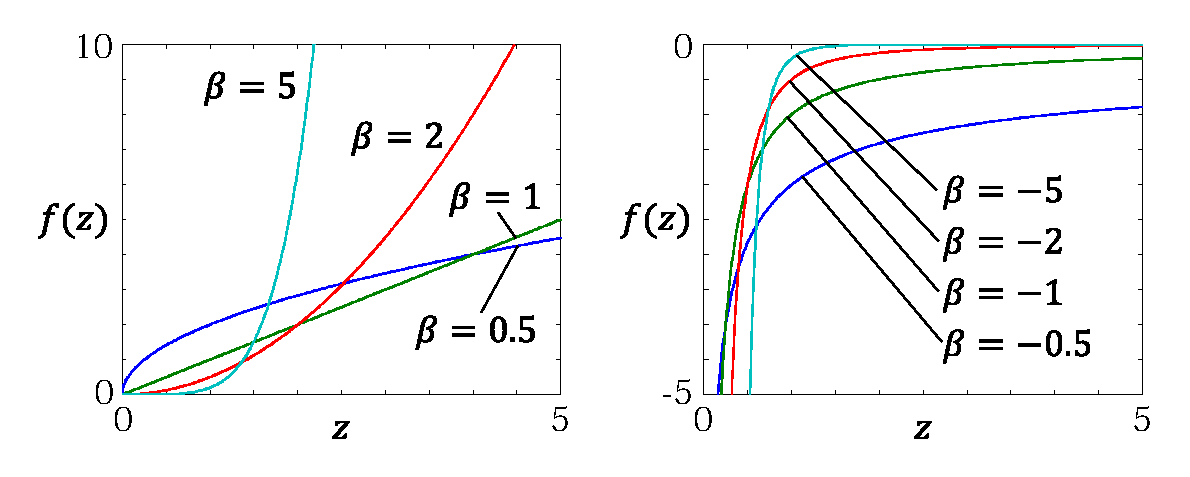
\includegraphics[width=.99\linewidth]{sections/factorization/beta_div_aux_functions}
\caption{いくつかの$\beta$に対する関数$f_\beta(z)=\frac{1}{\beta} z^\beta$のプロット.
$\beta=1$を境界として,$\beta \ge 1$のときは下に凸 (convex),$\beta \le 1$のときは上に凸 (concave) となることに注意.}
\label{fig:beta_div_aux_functions}
\end{figure}

まず,準備として,
関数$f_\beta(z)=\frac{1}{\beta} z^\beta \ (z > 0)$について考えます(\figref{fig:beta_div_aux_functions}).
$\beta \le 1$の場合は,$f_\beta(z)$は上に凸であることから,
任意の点$\omega > 0$における一次のテイラー展開
($\omega$における接線方程式)を考えることで,
$f_\beta(z)$の上限関数$u_\beta(z,\omega)$を設計できます.
\begin{align}
f_\beta(z)
\le
\frac{1}{\beta} \omega^\beta + \omega^{\beta - 1}\left(z - \omega\right)
=
\frac{\beta + 1}{\beta} \omega^\beta + \omega^{\beta - 1} z
\overset{\mbox{\scriptsize{def}}}{=}
u_\beta(z,\omega)
\end{align}
ここで,等号成立条件,すなわち,$u_\beta(z,\omega)$を最小化する$\omega$は,
$u_\beta(z,\omega)$を$\omega$で偏微分して$0$とおくことで求まります
(導出はEU-NMF, KL-NMF, IS-NMFなどと同様なので省略).
\begin{align}
\omega = x
\end{align}
一方,$\beta \ge 1$の場合は,$f_\beta(z)$は下に凸であることから,
Jensenの不等式を用いて,$f'_\beta(\bm{z}) = \frac{1}{\beta} \left(\sum_{k=1}^K z_k\right)^\beta$の
上限関数$u'_\beta(\bm{z},\bm\lambda)$を設計できます.
\begin{align}
f'_\beta(\bm{z}) 
= 
\frac{1}{\beta} \left(\sum_{k=1}^K \lambda_k \frac{z_k}{\lambda_k}\right)^\beta
\le 
\frac{1}{\beta} \sum_{k=1}^K \lambda_k \left(\frac{z_k}{\lambda_k}\right)^\beta
\overset{\mbox{\scriptsize{def}}}{=}
u'_\beta(\bm{z},\bm\lambda)
\end{align}
ここで,補助変数$\bm\lambda = \{\lambda_k\}_{k=1}^K$は,$\sum_{k=1}^K \lambda_k = 1$を満たします.
等号成立条件,すなわち,$u'_\beta(\bm{z},\bm\lambda)$を最小化する$\bm\lambda$は,
$u'_\beta(\bm{z},\bm\lambda)$を$\bm\lambda$で偏微分して$0$とおくことで求まります(導出は省略).
\begin{align}
\lambda_k = \frac{z_k}{\sum_{k=1}^K z_k}
\end{align}

また,関数$g'_\beta(\bm{z})
= - \frac{1}{\beta - 1} \left(\sum_{k=1}^K z_k\right)^{\beta - 1}$
および関数$g_\beta(z) = - \frac{1}{\beta - 1} z^{\beta - 1}$についても,
$g'_\beta(\bm{z}) = - f'_{\beta-1}(\bm{z})$
および$g_\beta(z) = - f_{\beta-1}(z)$となることを用いて,
上限関数をそれぞれ設計できます.
\begin{align}
g'_\beta(\bm{z}) &\le - u'_{\beta - 1}(\bm{z},\bm\lambda)
&(\beta \le 2)
\\
g_\beta(z) &\le - u_{\beta - 1}(z,\omega)
&(\beta \ge 2)
\end{align}
各場合における等号成立条件,すなわち,上限関数を最小化する
補助変数$\bm\lambda$あるいは$\omega$は,次式で与えられます.
\begin{align}
\lambda_k &= \frac{z_k}{\sum_{k=1}^K z_k} &(\beta \le 2)
\\
\omega &= x &(\beta \ge 2)
\end{align}

これらの結果を用いて,コスト関数$\mathcal{D}(\bm{X}|\bm{Y})$に対して,
補助変数$\bm\lambda$および$\bm\omega$を含む
上限関数$\mathcal{U}(\bm{X}|\bm{Y},\bm\lambda,\bm\omega)$を導出します.
\begin{align}
&\mathcal{D}(\bm{X}|\bm{Y}) 
\overset{c}{=}
\sum_{n=1}^N \sum_{m=1}^M 
\left(
\frac{1}{\beta} y_{nm}^\beta - x_{nm} \frac{1}{\beta - 1} y_{nm}^{\beta - 1}
\right)
\nonumber\\
&=
\left\{
\begin{array}{ll}
\sum_{n=1}^N \sum_{m=1}^M \left(u_\beta(y_{nm},\omega_{nm})           
- x_{nm} u'_{\beta - 1}(\bm{y}_{nm},\bm\lambda_{nm})\right) & (\beta < 1) \\
\sum_{n=1}^N \sum_{m=1}^M \left(u'_\beta(\bm{y}_{nm},\bm\lambda_{nm}) 
- x_{nm} u'_{\beta - 1}(\bm{y}_{nm},\bm\lambda_{nm})\right) & (1 \le \beta \le 2) \\
\sum_{n=1}^N \sum_{m=1}^M \left(u'_\beta(\bm{y}_{nm},\bm\lambda_{nm}) 
- x_{nm} u_{\beta - 1}(y_{nm},\omega_{nm})\right) & (\beta > 2)
\end{array}
\right.
\nonumber\\
&\overset{\mbox{\scriptsize{def}}}{=}
\mathcal{U}(\bm{X}|\bm{Y},\bm\lambda,\bm\omega)
\label{eqn:beta_nmf_u}
\end{align}
ここで,$\bm{y}_{nm} = \{y_{nmk}\}_{k=1}^K = \{w_{km}h_{kn}\}_{k=1}^K$,
$\bm\lambda_{nm} = \{\lambda_{nmk}\}_{k=1}^K$と定義しました.
いずれの場合においても,等号成立条件,
すなわち$\mathcal{U}(\bm{X}|\bm{Y},\bm\lambda,\bm\omega)$を最小化する
$\bm\lambda$および$\bm\omega$は次式で与えられます.
\begin{align}
\lambda_{nmk} 
&= \frac{w_{km}h_{kn}}{y_{nm}}
\label{eqn:beta_nmf_mu_lambda}
\\
\omega_{nm} &= y_{nm}
\label{eqn:beta_nmf_mu_omega}
\end{align}

最後に,$\mathcal{U}(\bm{X}|\bm{Y},\bm\lambda,\bm\omega)$を最小化する
$\bm{Y}$($\bm{W}$および$\bm{H}$)を求めます.
$\mathcal{U}(\bm{X}|\bm{Y},\bm\lambda,\bm\omega)$は,
$w_{km}$あるいは$h_{kt}$に関する一次導関数および二次導関数を計算することにより,
いずれの変数についても凸関数であることが分かります\cite{nakano:mlsp:2010}.
したがって,$\mathcal{U}(\bm{X}|\bm{Y},\bm\lambda,\bm\omega)$を$w_{km}$について
偏微分してゼロとおくことにより,$\bm{H}$が与えられたもとでの$w_{km}$の最適解が得られます.
\begin{align}
 w_{km} = 
 \left\{
 \begin{array}{ll}
  \left(
  \frac
   {\sum_{n=1}^N \lambda_{nmk}^{2 - \beta} x_{nm} h_{kn}^{\beta - 1}}
   {\sum_{n=1}^N \omega_{nm}^{\beta - 1} h_{kn}}
  \right)^{\frac{1}{2 - \beta}}
   &
   (\beta < 1)
   \\
  \frac
   {\sum_{n=1}^N \lambda_{nmk}^{2 - \beta} x_{nm} h_{kn}^{\beta - 1}}
   {\sum_{n=1}^N \omega_{nm}^{1 - \beta} h_{kn}^\beta}
   &
   (1 \le \beta \le 2)
   \\
  \left(
  \frac
   {\sum_{n=1}^N \lambda_{nmk}^{\beta - 2} x_{nm} h_{kn}}
   {\sum_{n=1}^N \omega_{nm}^{1 - \beta} h_{kn}^\beta}
  \right)^{\frac{1}{\beta - 1}}
   &
   (\beta > 2)
 \end{array}
 \right.
 \label{eqn:beta_nmf_mu_w}
\end{align}
補助関数を介さない乗法更新則は,\refeq{eqn:beta_nmf_mu_lambda}および
\refeq{eqn:beta_nmf_mu_omega}を\refeq{eqn:beta_nmf_mu_w}に代入することで得られます.
\begin{align}
w_{km} 
\gets 
   \left(
   \frac
   {\sum_{n=1}^N h_{kn} y_{nm}^{\beta - 2} x_{nm}}
   {\sum_{n=1}^N h_{kn} y_{nm}^{\beta - 1}}
   \right)^{\psi(\beta)}
 w_{km}
\end{align}
ここで,$\psi(\beta)$は$\beta$の関数であり,次式で与えられます.
\begin{align}
\psi(\beta) 
= 
\left\{
\begin{array}{ll}
\frac{1}{2 - \beta} & (\beta < 1)
\\
1 &  (1 \le \beta \le 2)
\\
\frac{1}{\beta - 1} & (\beta > 2)
\end{array}
\right.
\end{align}
$h_{kn}$の乗法更新則も同様にして導出できます.
\begin{align}
h_{kn} 
\gets 
   \left(
   \frac
   {\sum_{m=1}^M w_{km} y_{nm}^{\beta - 2} x_{nm}}
   {\sum_{m=1}^M w_{km} y_{nm}^{\beta - 1}}
   \right)^{\psi(\beta)}
 h_{kn}
\end{align}
さらに,これらは行列演算として簡潔に記述することもできます.
\begin{align}
\bm{W} \gets 
\left(
\frac{\bm{H} \left(\bm{X} \odot \bm{Y}^{\beta - 2}\right)^T}
                  {\bm{H} \left(\bm{Y}^{\beta - 1}\right)^T}
\right)^{\psi(\beta)}
 \odot \bm{W}
\label{eqn:beta_nmf_mu_W}
\\
\bm{H} \gets 
\left(
\frac{\bm{W} \left(\bm{X} \odot \bm{Y}^{\beta - 2}\right)^T}
                  {\bm{W} \left(\bm{Y}^{\beta - 1}\right)^T}
\right)^{\psi(\beta)}
 \odot \bm{H}
\label{eqn:beta_nmf_mu_H}
\end{align}
ここで,$\bm{Z}^\alpha$は,行列$\bm{Z}$の各要素を$\alpha$乗することを意味するものとします.

\begin{algobox}{$\beta$-NMFの最尤推定}
\label{algo:beta-nmf-ml}
\begin{algorithmic}[1]
\Require 非負値行列$\bm{X} \in \mathbb{R}_+^{M \times N}$, 基底数$K$,任意の実数$\beta$
\State 非負値行列$\bm{W} \in \mathbb{R}_+^{M \times K}$をランダムに初期化
\State 非負値行列$\bm{H} \in \mathbb{R}_+^{M \times K}$をランダムに初期化
\State $\psi(\beta) 
= 
\left\{
\begin{array}{ll}
\frac{1}{2 - \beta} & (\beta < 1)
\\
1 &  (1 \le \beta \le 2)
\\
\frac{1}{\beta - 1} & (\beta > 2)
\end{array}
\right.$
\While{上限関数$\mathcal{U}(\bm{X}|\bm{Y},\bm\lambda,\bm\omega)$が未収束}
\State $\displaystyle \bm{W} \gets 
\left(
\frac{\bm{H} \left(\bm{X} \odot \bm{Y}^{\beta - 2}\right)^T}
                  {\bm{H} \left(\bm{Y}^{\beta - 1}\right)^T}
\right)^{\psi(\beta)}
 \odot \bm{W}$ 
\State $\displaystyle \bm{H} \gets 
\left(
\frac{\bm{W} \left(\bm{X} \odot \bm{Y}^{\beta - 2}\right)^T}
                  {\bm{W} \left(\bm{Y}^{\beta - 1}\right)^T}
\right)^{\psi(\beta)}
 \odot \bm{H}$ 
\EndWhile\\
{\bf Return} 非負値行列$\bm{W}$, $\bm{H}$
\end{algorithmic}
\end{algobox}

\refalgo{algo:beta-nmf-ml}に,$\beta$-NMFのアルゴリズムを示します.
これは,
$\beta=2$とするとEU-NMFにおける\refalgo{algo:eu-nmf-ml}に,
$\beta=1$とするとKL-NMFにおける\refalgo{algo:kl-nmf-ml}に,
$\beta=0$とするとIS-NMFにおける\refalgo{algo:is-nmf-ml}に帰着することから,
統一的な乗法更新アルゴリズムとなっていることが分かります.

\subsection{乗法更新アルゴリズム}

NMFに対する乗法更新アルゴリズムは一意に定まるものではなく,
さまざまなバリエーションが存在します.
これまで紹介してきた補助関数法に基づく乗法更新アルゴリズム
(例:\refalgo{algo:beta-nmf-ml})は,
コスト関数の上限関数を導入し,上限関数を逐次最小化することにより,
もとのコスト関数を間接的に逐次最小化することができます.
さらに,収束性が保証されているという好ましい性質をもちます.
ただし,このようにして得られた反復更新則が,
乗法更新型の形式をとっていたことは必然的ではありません.
つまり,私たちは最初から乗法更新則を導出しようと考えていたわけではなく,
あくまで補助関数法に基づくコスト関数最小化の枠組みに従った結果,
たまたま乗法更新則が得られたということです.

本節では,より直接的にNMFの乗法更新則を導出するアプローチについて説明します.
研究コミュニティにおいて,
乗法更新則といえば,このアプローチで導出されたものを指すことが一般的です.
しかし,必ずしも最も好ましい乗法更新則になっているとは限らないことに注意が必要です.
まず,多くの場合で,このアプローチで導出される乗法更新則には収束性が保証されていません.
また,経験的にはほとんどの場合で収束するとしても,
収束速度が最も高速であるとも限りません.

具体的に,$\beta$-NMFの乗法更新則を導出してみましょう.
まず,最小化すべきコスト関数は次式で与えられます.
\begin{align}
\mathcal{D}(\bm{X}|\bm{Y}) 
\overset{c}{=}
\sum_{n=1}^N \sum_{m=1}^M 
\left(
\frac{1}{\beta} y_{nm}^\beta - x_{nm} \frac{1}{\beta - 1} y_{nm}^{\beta - 1}
\right)
\end{align}
私たちの目的は,$\mathcal{D}(\bm{X}|\bm{Y})$を
逐次最小化するような乗法更新則
\begin{align}
 w_{km} &\gets \eta_{km} w_{km}
 \\
 h_{kn} &\gets \zeta_{kn} h_{kn}
\end{align}
を見つけることです.

適切な係数$\eta_{km}$および$\zeta_{kn}$を求めるには,
まず,$\mathcal{D}(\bm{X}|\bm{Y})$を$w_{km}$について偏微分します.
\begin{align}
\frac{\partial \mathcal{D}(\bm{X}|\bm{Y})}{\partial w_{km}}
&=
\frac{\partial \mathcal{D}(\bm{X}|\bm{Y})}{\partial y_{nm}}
\frac{\partial y_{nm}}{\partial w_{km}}
\nonumber\\
&=
\sum_{n=1}^N y_{nm}^{\beta - 1} h_{kn}
-
\sum_{n=1}^N x_{nm} y_{nm}^{\beta - 2} h_{kn}
\nonumber\\
&\overset{\mbox{\scriptsize def}}{=} \kappa_{km}^+ - \kappa_{km}^-
\label{eqn:beta_nmf_pdiv}
\end{align}
ここで,$y_{nm} = \sum_{k=1}^K w_{km} h_{kn}$であることを用いました.
\refeq{eqn:beta_nmf_pdiv}では,
第一項$\kappa_{km}^+$および第二項$\kappa^-_{km}$はいずれも非負値であることから,
$\mathcal{D}(\bm{X}|\bm{Y})$の偏微分が,
二つの非負値の差によって表現されていることが分かります.
ここで,$\kappa_{km}^+$を分母に,$\kappa_{km}^-$を分子として,$\eta_{km}$を
\begin{align}
\eta_{km} 
= \frac{\kappa_{km}^-}{\kappa_{km}^+} 
= \frac{\sum_{n=1}^N x_{nm} y_{nm}^{\beta - 2} h_{kn}}{\sum_{n=1}^N y_{nm}^{\beta - 1} h_{kn}}
\label{eqn:mu_eta_km}
\end{align}
で計算することにします.


$h_{kn}$についても同様であり,
最終的に得られる乗法更新則を行列演算形式で記述すると以下の通りです.
\begin{align}
\bm{W} \gets 
\frac{\bm{H} \left(\bm{X} \odot \bm{Y}^{\beta - 2}\right)^T}
                  {\bm{H} \left(\bm{Y}^{\beta - 1}\right)^T}
 \odot \bm{W}
\label{eqn:beta_nmf_mu_W_2}
\\
\bm{H} \gets 
\frac{\bm{W} \left(\bm{X} \odot \bm{Y}^{\beta - 2}\right)^T}
                  {\bm{W} \left(\bm{Y}^{\beta - 1}\right)^T}
 \odot \bm{H}
\label{eqn:beta_nmf_mu_H_2}
\end{align}
これらの乗法更新則については,$1 \le \beta \le 2$のときに限り,
収束性が証明されています.
\refeq{eqn:beta_nmf_mu_W_2}および\refeq{eqn:beta_nmf_mu_H_2}と,
\refeq{eqn:beta_nmf_mu_W}および\refeq{eqn:beta_nmf_mu_H}を比較すると,
係数部分に$\psi(\beta)$乗がかかっているかどうかの違いがあります.

\section{非負値行列因子分解の確率的な解釈}

NMFは最尤推定であってもスパースな解が得られやすいが,
適切な事前分布を導入してベイズ推定を行うことで,
よりスパースな解を得ることができる.
更に,ノンパラメトリックベイズモデルを定式化すれば,
基底数を$K \rightarrow \infty$とした場合でもスパースな学習が可能になる.
すなわち,観測行列$\bm{X}$に合わせて
高々有限個の基底がアクティベートされるような機構が実現できる.
具体的には,ガンマ過程あるいはベータ過程を事前分布に用いることになる.

\subsection{確率モデルの最尤推定としての定式化}

\subsection{ノンパラメトリックベイズモデル}

\begin{figure}[t]
\centering
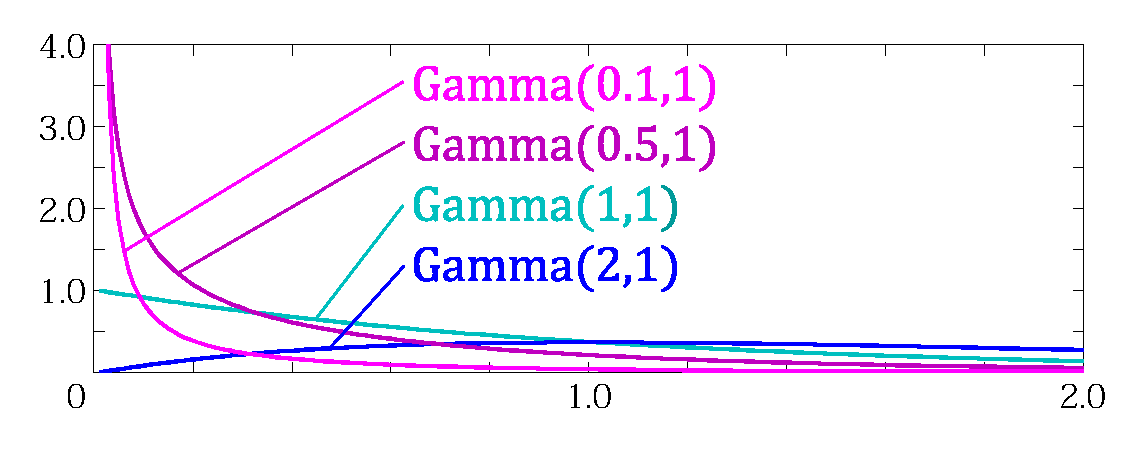
\includegraphics[width=.9\linewidth]{sections/factorization/gamma}
\caption{形状母数が異なる幾つかのガンマ分布.}
\label{fig:gamma}
\end{figure}

ガンマ過程に基づくNMFのノンパラメトリックベイズモデル (GaP-NMF)について説明する.
まず,\refeq{eqn:x_wh_elem}に対し,
$K$次元の非負値ベクトル
$\bm\theta = [\theta_1,\theta_2,\cdots,\theta_K]$を導入する.
\begin{align}
 \bm{x}_n \approx 
 \sum_{k=1}^{K} \theta_k h_{kn} \bm{w}_k \overset{\mbox{\tiny def}}{=} \bm{y}_n
\end{align}
ここで,$\theta_k \ge 0$は基底$k$の大域的な重みである.
この$\bm\theta$に対し,
観測データ$\bm{X}$を表現するのに必要な基底$k$以外の要素$\theta_k$が
ゼロとなるようなスパースな学習を行いたい.

ノンパラメトリックベイズモデルを定式化するため,
$\bm\theta$,$\bm{W}$,$\bm{H}$に対して事前分布を導入する.
まず,$\bm{W}$及び$\bm{H}$の各要素は非負値であるので,
ガンマ事前分布を用いると都合が良い.
\begin{align}
w_{km} &\sim \mbox{Gamma}(a_0^w, b_0^w)
\label{eqn:p_w_km}
\\
h_{kn} &\sim \mbox{Gamma}(a_0^h, b_0^h)
\label{eqn:p_h_kn}
\end{align}
ここで,$a_0^* > 0$及び$b_0^* > 0$はそれぞれ,
ガンマ分布の形状母数と逆尺度母数である.
更に,$\bm\theta$に対しても同様にガンマ事前分布を仮定する.
\begin{eqnarray}
 \theta_k \sim \mbox{Gamma}\left(\frac{\alpha c}{K}, \alpha\right)
  \label{eqn:p_t_k}
\end{eqnarray}
ここで,$\alpha > 0$及び$c > 0$は超パラメータである.
ガンマ分布の形状母数が小さくなるほど0が出る確率が大きくなる(\figref{fig:gamma}).
ただし,$\mathbb{E}_{\mbox{\scriptsize prior}}[\theta_k] = \frac{c}{K}$,
$\mathbb{E}_{\mbox{\scriptsize prior}}[\sum_k \theta_k] = c$である.

ここで,\refeq{eqn:p_w_km},\refeq{eqn:p_h_kn}及び\refeq{eqn:p_t_k}で構成される
有限モデルに対して,$K \rightarrow \infty$となる極限を考えると,
以下のガンマ過程が得られる.
\begin{eqnarray}
G \sim \mbox{GaP}(\alpha, G_0)
\end{eqnarray}
ここで,$G_0$は空間$U$($\bm{w} \in \mathbb{R}_+^M$と$\bm{h} \in \mathbb{R}_+^N$の直積空間)上に
定義された基底測度であり,$G_0(U) = c$を満たす(\figref{fig:gap}).
このとき,$G$は$U$上の離散測度となり,
空間$U$の任意の分割$\{U_i\}_{i=1}^I$に対して
\begin{align}
G(U_i) \sim \mbox{Gamma}(\alpha G_0(U_i), \alpha)
\end{align}
が成立している.ただし,$\mathbb{E}[G] = G_0$である.
微小区間への分割を$\{U_k\}_{k=1}^\infty$とすると,
$G(U_k) = \theta_k$である.
$\alpha$は集中度と呼ばれ,$\alpha$が小さくなるほど$\bm\theta$は
よりスパースになる.
計算機上では$K \rightarrow \infty$は扱えないが,
$K$を$\alpha$に比べて十分大きな値に設定すれば,
\refeq{eqn:p_t_k}はガンマ過程の良い近似となる(weak-limit approximation).
%この他,棒折り過程など他の構成法も利用可能と考えられる.

\begin{algorithm}[t]
\caption{GaP-KL-NMFのベイズ推定}
\label{kl-nmf-vb}
\begin{algorithmic}[1]
\Require 非負値行列$\bm{X} \in \mathbb{R}_+^{M \times N}$, 
最大基底数$K$,ガンマ過程の集中度$\alpha$,
ガンマ分布のパラメータ$a_0^w,b_0^w,a_0^h,b_0^h$
\State 変分事後分布$q(\bm\theta)$, $q(\bm{W})$, $q(\bm{H})$をランダムに初期化
\While{not converged}
\State $\lambda_{knm} \propto \mathbb{E}_{q}[\theta_k w_{km} h_{kn}]$
\State $\textstyle q(\theta_k)
= \mbox{Gamma}(\frac{\alpha c}{K} + \sum_{nm} \lambda_{knm} x_{nm},$\\
\ \ \ \ \ \ \ \ \ \ \ \ \ \ \ \ \ \ \ \ \ \ \ \ \ \ \ $\alpha + \sum_{nm} \mathbb{E}_{q}[w_{km} h_{kn}])$
\State $\textstyle q(w_{km}) 
= \mbox{Gamma}(a_0^w + \sum_{n} \lambda_{knm} x_{nm},$\\
\ \ \ \ \ \ \ \ \ \ \ \ \ \ \ \ \ \ \ \ \ \ \ \ \ \ \ \ \ \ $b_0^w + \sum_{n} \mathbb{E}_{q}[\theta_k h_{kn}])$
\State $\textstyle q(h_{kn}) 
= \mbox{Gamma}(a_0^h + \sum_{m} \lambda_{knm} x_{nm},$\\
\ \ \ \ \ \ \ \ \ \ \ \ \ \ \ \ \ \ \ \ \ \ \ \ \ \ \ \ \ $b_0^h + \sum_{m} \mathbb{E}_{q}[\theta_k w_{km}])$
\EndWhile\\
{\bf Return} 変分事後分布$q(\bm\theta)$, $q(\bm{W})$, $q(\bm{H})$
\end{algorithmic}
\end{algorithm}

\subsection{GaP-KL-NMFのベイズ推定}
\label{sec:gap-kl-nmf}

まず,GaP-KL-NMFに対するVBを導出する.
\refeq{eqn:lb}で与えられる変分下限$\mathcal{L}(q)$の第一項は
\refeq{eqn:kl_s_p}で計算できる対数ポアソン尤度の期待値であるが,
依然として解析的に計算できない.
そのため,凹関数$f(x)=\log(x)$に対してJensenの不等式を用いると
更なる変分下限
\begin{align}
&
\mathbb{E}_{q}[\log p(\bm{X}|\bm\theta,\bm{W},\bm{H})]
\nonumber\\
&
\overset{c}{=} \mathbb{E}_{q}\!\!\left[\sum_{nm} \left(x_{nm} \log \sum_k y_{knm} - \sum_k y_{knm}\right)\right]
\nonumber\\
&
= \sum_{nm} x_{nm} \mathbb{E}_{q}\!\!\left[\log \sum_k \lambda_{knm} \frac{y_{knm}}{\lambda_{knm}}\right] 
&
\nonumber\\
& \ \ \ \
- \sum_{knm} \mathbb{E}_{q}\!\left[y_{knm}\right]
\nonumber\\
%\end{align}
%
%\begin{align}
&
\ge \sum_{nm} x_{nm} \sum_k \lambda_{knm} \mathbb{E}_{q}\!\!\left[\log \frac{y_{knm}}{\lambda_{knm}}\right] 
&
\nonumber\\
& \ \ \ \ 
- \sum_{knm} \mathbb{E}_{q}\!\left[y_{knm}\right]
\nonumber\\
&\overset{\mbox{\scriptsize def}}{=} 
\mathbb{E}_{q}[\log q(\bm{X}|\bm\theta,\bm{W},\bm{H})]
\label{eqn:lb2_kl}
\end{align}
を得る.ここで,$\lambda_{knm}$は$\sum_k \lambda_{knm} = 1$を満たす補助変数である.
等号成立条件(変分下限が最大となる条件)はラグランジュの未定乗数法を用いて求めることができ,
$\lambda_{knm} \propto \mathbb{E}_{q}[y_{knm}]$となる.

\begin{algorithm}[t]
\caption{GaP-IS-NMFのベイズ推定}
\label{is-nmf-vb}
\begin{algorithmic}[1]
\Require 非負値行列$\bm{X} \in \mathbb{R}_+^{M \times N}$, 最大基底数$K$,ガンマ過程の集中度$\alpha$,
ガンマ分布のパラメータ$a_0^w,b_0^w,a_0^h,b_0^h$
\State 変分事後分布$q(\bm\theta)$, $q(\bm{W})$, $q(\bm{H})$をランダムに初期化
\While{not converged}
\State $\lambda_{knm} \propto \mathbb{E}_{q}[\theta_k^{-1} w_{km}^{-1} h_{kn}^{-1}]^{-1}$
\State $\omega_{nm} \propto \sum_k \mathbb{E}_{q}[\theta_k w_{km} h_{kn}]$
\State $\textstyle q(\theta_k)
= \mbox{GIG}(\frac{\alpha c}{K}, 
\alpha + \sum_{nm} \omega_{nm}^{-1} \mathbb{E}_{q}\!\left[w_{km}\right] \mathbb{E}_{q}\!\left[h_{kn}\right],$\\
\ \ \ \ \ \ \ \ \ \ \ \ \ \ \ \ \ \ \ \ \ \ \ \ \ \ \ \ \
$\sum_{nm} x_{nm} \lambda_{knm}^2 \mathbb{E}_{q}\!\left[w_{mk}^{-1}\right] \mathbb{E}_{q}\!\left[h_{kn}^{-1}\right])$
\State $\textstyle q(w_{km})
= \mbox{GIG}(a_0^w, 
b_0^w + \sum_{n} \omega_{nm}^{-1} \mathbb{E}_{q}\!\left[\theta_k\right] \mathbb{E}_{q}\!\left[h_{kn}\right],$\\
\ \ \ \ \ \ \ \ \ \ \ \ \ \ \ \ \ \ \ \ \ \ \ \ \ \ \ 
$\sum_{n} x_{nm} \lambda_{knm}^2 \mathbb{E}_{q}\!\left[\theta_k^{-1}\right] \mathbb{E}_{q}\!\left[h_{kn}^{-1}\right])$
\State $\textstyle q(h_{kn})
= \mbox{GIG}(a_0^h, 
\sum_{m} \omega_{nm}^{-1} \mathbb{E}_{q}\!\left[\theta_k\right] \mathbb{E}_{q}\!\left[w_{km}\right],$\\
\ \ \ \ \ \ \ \ \ \ \ \ \ \ \ \ \ \ \ \ \ \ \ \
$\sum_{m} x_{nm} \lambda_{knm}^2 \mathbb{E}_{q}\!\left[\theta_k^{-1}\right] \mathbb{E}_{q}\!\left[w_{km}^{-1}\right]$)
\EndWhile\\
{\bf Return} 変分事後分布$q(\bm\theta)$, $q(\bm{W})$, $q(\bm{H})$
\end{algorithmic}
\end{algorithm}

最後に,各パラメータに対する変分事後分布を導出する.
実際には\refeq{eqn:lb}で与えられる元の変分下限$\mathcal{L}(q)$ではなく,
\refeq{eqn:lb2_kl}を用いて得られた更なる変分下限を最大化することになる.
その結果,\refeq{eqn:q_t}, (\ref{eqn:q_w}), (\ref{eqn:q_h})において,
$\log p(\bm{X},\bm\theta,\bm{W},\bm{H})$の代わりに
次式を用いることになる.
\begin{eqnarray}
\log q(\bm{X},\bm\theta,\bm{W},\bm{H}) 
= \log q(\bm{X}|\bm\theta,\bm{W},\bm{H})
\nonumber\\
+ \log p(\bm\theta) + \log p(\bm{W}) + \log p(\bm{H})
\end{eqnarray}
具体的には,最適な変分事後分布$q(\bm\theta)$は,$\bm\theta$に関連する項のみを取り出すと
以下の通り計算できる.
\begin{align}
\log q(\bm\theta) 
&\overset{c}{=}
\sum_{knm} x_{nm} \lambda_{knm} \log \theta_k
\nonumber\\
&
- \sum_{knm} \theta_k \mathbb{E}_{q}\!\left[w_{km}\right] \mathbb{E}_{q}\!\left[h_{kn}\right]
\nonumber\\
&
+ \sum_{k} \left( \left(\frac{\alpha c}{K} - 1\right) \log \theta_k - \alpha \theta_k \right)
\end{align}
従って,$\theta_k$の事後分布はガンマ分布となる.
同様に,最適な$q(\bm{W})$や$q(\bm{H})$もガンマ分布として求まる.
{\bf Algorithm \ref{kl-nmf-vb}}に更新則を示す.
反復ごとに,$\mathbb{E}[\theta_k]$が十分に小さい基底$k$を削除していけば,
実効的な基底数$K_+$が自動的に定まる.

\subsection{GaP-IS-NMFのベイズ推定}

次に,GaP-IS-NMFに対するVB\cite{hoffman:icml:2010}を導出する.
\refeq{eqn:lb}で与えられる変分下限$\mathcal{L}(q)$の第一項は
\refeq{eqn:is_p}で与えられる対数指数尤度の期待値であり,
やはり解析的に計算できない.
そこで,凹関数$f(x) = - \frac{1}{x}$に対してJensenの不等式を考える.
\begin{align}
- \frac{1}{\sum_{k=1}^K x_k} 
= - \frac{1}{\sum_{k=1}^K \lambda_k \frac{x_k}{\lambda_k}} \ge \sum_{k=1}^K \frac{\lambda_k^2}{x_k}
\end{align}
ここで,$\lambda_k$は$\sum_k \lambda_k = 1$を満たす補助変数であり,
等号成立条件は$\lambda_k \propto x_k$である.
更に,凸関数$g(x) = - \log(x)$に対する1次のテイラー展開($\omega$における接線)を考える.
\begin{align}
- \log (x) \ge - \log (\omega) - \frac{x}{\omega} + 1
\end{align}
ここで,$\omega$は補助変数であり,等号成立条件は$\omega = x$である.
これら二つの不等式を用いると
変分下限$\mathbb{E}_{q}[\log q(\bm{X}|\bm\theta,\bm{W},\bm{H})]$を得る.
\begin{align}
&
\mathbb{E}_{q}[\log p(\bm{X}|\bm\theta,\bm{W},\bm{H})]
\nonumber\\
&
\overset{c}{=} \mathbb{E}_{q}\!\!\left[\sum_{nm} 
\left(- x_{nm} \left(y_{nm}\right)^{-1} - \log \left(y_{nm}\right)\right)\right]
\nonumber\\
&
\ge - \sum_{nm} x_{nm} \mathbb{E}_{q}\!\!\left[\sum_k \frac{\lambda_{knm}^2}{y_{knm}}\right] 
\nonumber\\
&\ \ \
- \sum_{nm} \left(\log(\omega_{nm}) + \mathbb{E}_{q}\!\!\left[\frac{y_{nm}}{\omega_{nm}}\right] - 1\right)
\nonumber\\
&
\overset{\mbox{\scriptsize def}}{=} \mathbb{E}_{q}[\log q(\bm{X}|\bm\theta,\bm{W},\bm{H})]
\label{eqn:lb2_is}
\end{align}

各パラメータに対する変分事後分布は,\refsubsec{sec:gap-kl-nmf}と同様に求められる.
具体的には,最適な変分事後分布$q(\bm\theta)$は,$\bm\theta$に関連する項のみを取り出すと
\begin{align}
&
\log q(\bm\theta) 
\overset{c}{=} 
- \sum_{knm} x_{nm} \lambda_{knm}^2 \theta_k^{-1} \mathbb{E}_{q}\!\!\left[w_{km}^{-1}\right] \mathbb{E}_{q}\!\!\left[h_{kn}^{-1}\right] 
\nonumber\\
&\ \
- \sum_{knm} \omega_{nm}^{-1} \theta_k \mathbb{E}_{q}\!\left[w_{km}\right] \mathbb{E}_{q}\!\left[h_{kn}\right]
\nonumber\\
&\ \ \ \
+ \sum_{k} \left( \left(\frac{\alpha c}{K} - 1\right) \log \theta_k - \alpha \theta_k \right)
\end{align}
従って,$\theta_k$の事後分布はGeneralized Inverse Gaussian (GIG) 分布となることが分かる
(詳細は\cite{hoffman:icml:2010}参照).
{\bf Algorithm \ref{is-nmf-vb}}に更新則を示す.

\subsection{BP-KL-NMFのベイズ推定}


\section{半正定値テンソル分解}

このような無限次元の空間($K\rightarrow\infty$)におけるスパースな学習は,
ノンパラメトリックベイズモデルを用いて実現することができる\cite{hoffman:icml:2010}.
近年,NMFの数学的に自然な拡張である半正定値テンソル分解 
(Positive Semidefinite Tensor Factorization: PSDTF)\cite{yoshii:icml:2013,yoshii:ismir:2013}が提案され,
優れた音源分離結果を達成している.

本章では,NMFの自然な拡張である
半正定値テンソル分解\cite{yoshii:icml:2013,yoshii:ismir:2013}(PSDTF) について解説する.
PSDTFでは,各フレーム$n$の複素スペクトル$\tilde{\bm{x}}_n$の
自己共分散$\bm{X}_n \!=\! \tilde{\bm{x}}_n\tilde{\bm{x}}_n^H$,
すなわち{\bf 半正定値行列を少数の半正定値行列の和に分解}する(\figref{fig:comparison}).
一方,NMFでは,上記行列の対角成分(パワースペクトル)
$\bm{x}_n \!=\! \tilde{\bm{x}}_n \odot \tilde{\bm{x}}_n^*$,すなわち
{\bf 非負値ベクトルを少数の非負値ベクトルの和に分解}する.
行列の半正定値性はベクトルの非負値性の拡張概念であり,
非負値テンソル分解 (Nonnegative Tensor Factorization: NTF) と
PSDTFとは異なる.

音源分離においては,観測スペクトログラム$\tilde{\bm{X}}$から,
\refeq{eqn:s}を満たす音源スペクトログラム$\tilde{\bm{X}}_k$の位相を推定できる.
音源信号の周期と短時間フーリエ変換の窓長$M$が異なると,
音源信号の巡回定常性の仮定が成り立たないため,
周波数ビン間の相関を取り扱える利点は大きい.
マルチチャネル音源分離において,
%周波数ビン間の相関行列ではなく,
マイク間の相関行列を分解する際にも同様のモデルが提案されている\cite{sawada:ieee:2013}.

\subsection{コスト関数最小化としての定式化}
\label{sec:ps}

\begin{figure}[t]
\centering
\includegraphics[width=\columnwidth]{sections/factorization/comparison}
\caption{音源分離のための半正定値テンソル分解 (PSDTF).}
\label{fig:comparison}
\end{figure} 

PSDTFでは,観測データとして3階のテンソル
$\bm{X} = [\bm{X}_1,\cdots,\bm{X}_n] \in \mathbb{C}^{M \times M \times N}$
に対する分解を行う.
各要素$\bm{X}_n \succeq \bm{0} \in \mathbb{C}^{M \times M}$は半正定値行列とする.
今,各$\bm{X}_n$を
$K$個の半正定値行列$\{\bm{W}_k\}_{k=1}^{K}$(基底行列)
の凸結合で近似したい.
\begin{align}
 \bm{X}_{n} \approx 
  \sum_{k=1}^{K} h_{kn} \bm{W}_k
  \overset{\mbox{\tiny def}}{=} \bm{Y}_n
 \label{eqn:x_n_psdtf}
\end{align}
ここで,$h_{kn} \ge 0$は$\bm{X}_n$における
基底行列$\bm{W}_k$の重みである.
観測行列$\bm{X}_n$と再構成行列$\bm{Y}_n$との間の誤差$\mathcal{D}(\bm{X}_n|\bm{Y}_n)$を
評価する尺度として,非負値ベクトル間のKLダイバージェンスや
ISダイバージェンスの拡張である,
半正定値行列間のvon-Neumann (vN) ダイバージェンスや
Log-Determinant (LD) ダイバージェンスがある\cite{kulis:jmlr:2009}.
\begin{align}
 &
 \mathcal{D}_{\mbox{\tiny vN}}(\bm{X}_n|\bm{Y}_n)
 = \mbox{tr}\left(\bm{X}_n \log \bm{X}_n - \bm{X}_n \log \bm{Y}_n\right.
 \nonumber\\
 & \ \ \ \ \ \ \ \ \ \ \ \ \ \ \ \ \ \ \ \ \ \
 \left.- \bm{X}_n + \bm{Y}_n\right)
 \label{eqn:psdtf_vn}\\
 &
 \mathcal{D}_{\mbox{\tiny LD}}(\bm{X}_n|\bm{Y}_n)
 = \mbox{tr}\left(\bm{X}_n \bm{Y}_n^{-1}\right)
 \nonumber\\
 & \ \ \ \ \ \ \ \ \ \ \ \ \ \ \ \ \ \ \ \ \ \
 - \log\left|\bm{X}_n \bm{Y}_n^{-1}\right|
 - M
 \label{eqn:psdtf_ld}
\end{align}

\subsection{乗法更新アルゴリズムに基づく最適化}
\label{sec:psdtf_mu}

コスト関数$\mathcal{D}(\bm{X}|\bm{Y})
 =\sum_n \mathcal{D}(\bm{X}_n|\bm{Y}_n)$
を最小化する
$\bm{H} = [\bm{h}_1,\cdots,\bm{h}_K] \in \mathbb{R}^{N \times K}$
及び$\bm{W} = [\bm{W}_1,\cdots,\bm{W}_K] \in \mathbb{C}^{M \times M \times K}$
を求めるため,LD-PSDTFに対しても%補助関数法に基づく収束性が保証された
乗法更新アルゴリズム\cite{yoshii:ismir:2013,yoshii:icml:2013}が提案されている.
更新則は{\bf Algorithm?\ref{ld-psdtf-ml}}で与えられる
(導出は文献\cite{yoshii:ismir:2013,yoshii:icml:2013}参照).
$h_{kn}$の非負性と
$\bm{W}_k$の半正定値性は自然に保たれているが,
$\mbox{tr}(\bm{W}_k)=1$を満たすよう,反復ごとに
$\bm{W}_k$及び$\bm{h}_k$をスケーリングしておく.
%{\bf Algorithm?\ref{ld-psdtf-ml}}は,
%{\bf Algorithm?\ref{is-nmf-ml}}の自然な拡張である.

\section{確率的潜在成分解析}

Probabilitic Latent Component Analysis

\subsection{確率モデルの最尤推定としての定式化}

\subsection{ノンパラメトリックベイズモデル}

\subsection{音源分離への応用}

前節の議論を踏まえて,\refeq{eq:kl_s_p}, (\ref{eq:p_w_km}),
(\ref{eq:p_h_kn}), (\ref{eq:p_t_k})で定義される
ノンパラメトリックベイズKL-NMF (GaP-KL-NMF)
あるいは\refeq{eq:is_s_p}, (\ref{eq:p_w_km}),
        (\ref{eq:p_h_kn}), (\ref{eq:p_t_k})で定義される
ノンパラメトリックベイズIS-NMF (GaP-IS-NMF)に対する
変分ベイズ法 (Variational Bayes: VB) について述べる.
今,観測データ$\bm{X}$が与えられたときに,
ベイズの定理を用いて未知パラメータ$\bm\theta,\bm{W},\bm{H}$の事後分布
\begin{eqnarray}
 p(\bm\theta,\bm{W},\bm{H} | \bm{X}) 
 = \frac{p(\bm{X}, \bm\theta,\bm{W},\bm{H})}{p(\bm{X})}
\end{eqnarray}
を計算したい.
しかし,周辺尤度$p(\bm{X})$は解析的に計算できないため,
対数周辺尤度の変分下限$\mathcal{L}(q)$を構成し,
逐次最大化を行うことで$p(\bm{X})$を近似することを考える.
すなわち,変分分布$q(\bm\theta,\bm{W},\bm{H})$に対し,
凹関数$f(x)=\log(x)$に対してJensenの不等式を用いると以下を得る.
\begin{align}
&
 \log p(\bm{X})
 \nonumber\\
&
 = \log \int q(\bm\theta,\bm{W},\bm{H}) 
 \frac{p(\bm{X},\bm\theta,\bm{W},\bm{H})}{q(\bm\theta,\bm{W},\bm{H})} d\bm\theta d\bm{W} d\bm{H}
 \nonumber\\
&
 \ge \int q(\bm\theta,\bm{W},\bm{H}) 
 \log \frac{p(\bm{X},\bm\theta,\bm{W},\bm{H})}{q(\bm\theta,\bm{W},\bm{H})} d\bm\theta d\bm{W} d\bm{H}
 \nonumber\\
&
 = \mathbb{E}_{q(\bm\theta,\bm{W},\bm{H})}[\log p(\bm{X},\bm\theta,\bm{W},\bm{H})]
 \nonumber\\
& \ \ \ \
 - \mathbb{E}_{q(\bm\theta,\bm{W},\bm{H})}[\log q(\bm\theta,\bm{W},\bm{H})]
 \nonumber\\
&
 \overset{\mbox{\scriptsize def}}{=} \mathcal{L}(q)
\end{align}
等号成立条件は$q(\bm\theta,\bm{W},\bm{H}) = p(\bm\theta,\bm{W},\bm{H}|\bm{X})$であり,
このとき$\mathcal{L}(q)$が最大値をとる.
しかし,真の事後分布$p(\bm\theta,\bm{W},\bm{H} | \bm{X})$は計算困難であるため,
変分事後分布を因子分解可能な形$q(\bm\theta,\bm{W},\bm{H}) = q(\bm\theta) q(\bm{W}) q(\bm{H})$に限定し,
その中でも以下で計算できる変分下限
\begin{align}
&
 \mathcal{L}(q) = \mathbb{E}_{q}[\log p(\bm{X}|\bm\theta,\bm{W},\bm{H})]
 + \mathbb{E}_{q}[\log p(\bm\theta)]
 \nonumber\\
& \ \ \ \
 + \mathbb{E}_{q}[\log p(\bm{W})]
 + \mathbb{E}_{q}[\log p(\bm{H})]
 \nonumber\\
& \ \ \ \
 + H(q(\bm\theta)) + H(q(\bm{W})) + H(q(\bm{H}))
 \label{eq:lb}
\end{align}
を最大化するものを求めたい.
ここで,$H(\cdot)$はエントロピーを表す.
これは,変分事後分布$q(\bm\theta) q(\bm{W}) q(\bm{H})$の
真の事後分布$p(\bm\theta,\bm{W},\bm{H}|\bm{X})$に対するKLダイバージェンスを最小化することと等価である.
\refeq{eq:lb}を逐次最大化するには,
以下の更新式を収束するまで繰り返せば良い.
\begin{eqnarray}
 \!\!
 q(\bm\theta) \propto \exp(\mathbb{E}_{q(\bm{H},\bm{W})}[\log p(\bm{X},\bm\theta,\bm{W},\bm{H})])
 \label{eq:q_t}
 \\
 \!\!
 q(\bm{H}) \propto \exp(\mathbb{E}_{q(\bm\theta,\bm{W})}[\log p(\bm{X},\bm\theta,\bm{W},\bm{H})])
 \label{eq:q_w}
 \\
 \!\!
 q(\bm{W}) \propto \exp(\mathbb{E}_{q(\bm\theta,\bm{H})}[\log p(\bm{X},\bm\theta,\bm{W},\bm{H})]) 
 \label{eq:q_h}
\end{eqnarray}
